
\appendix
\chapter*{Appendix: User manual for gftest}
\addcontentsline{toc}{chapter}{Appendix: User manual for gftest}

\makeatother
% Scale images if necessary, so that they will not overflow the page
% margins by default, and it is still possible to overwrite the defaults
% using explicit options in \includegraphics[width, height, ...]{}
\setlength{\emergencystretch}{3em}  % prevent overfull lines
\providecommand{\tightlist}{%
  \setlength{\itemsep}{0pt}\setlength{\parskip}{0pt}}
\setcounter{secnumdepth}{0}
% Redefines (sub)paragraphs to behave more like sections
\ifx\paragraph\undefined\else
\let\oldparagraph\paragraph
\renewcommand{\paragraph}[1]{\oldparagraph{#1}\mbox{}}
\fi
\ifx\subparagraph\undefined\else
\let\oldsubparagraph\subparagraph
\renewcommand{\subparagraph}[1]{\oldsubparagraph{#1}\mbox{}}
\fi






% \hypertarget{gftest-automatic-test-case-generation-for-gf-grammars}{%
% \section{gftest: Automatic test case generation for GF
% grammars}\label{gftest-automatic-test-case-generation-for-gf-grammars}}

\noindent \texttt{gftest} is a program for automatically generating systematic
test cases for GF grammars. The basic use case is to give
\texttt{gftest} a PGF grammar, a concrete language and a function; then
\texttt{gftest} generates a representative and minimal set of example
sentences for a human to look at.
There are examples of actual generated test cases later in this
document, as well as the full list of options to give to
\texttt{gftest}.
\textbf{It is recommended to compile your PGF with the gf flag
\texttt{-\/-optimize-pgf}}, otherwise this tool can be very slow. For
example, \texttt{gf\ -make\ -\/-optimize-pgf\ LangEng.gf}.

A live version of this user manual is found at \url{https://github.com/GrammaticalFramework/gftest#readme}. The version in this thesis is from October 2018.

\hypertarget{table-of-contents}{%
\subsection{Table of Contents}\label{table-of-contents}}

\begin{itemize}
\tightlist
\item
  \protect\hyperlink{installation}{Installation}

\item
  \protect\hyperlink{common-use-cases}{Common use cases}

  \begin{itemize}
  \tightlist
  \item[$\circ$]
    \protect\hyperlink{grammar--g}{Grammar: \texttt{-g}}
  \item[$\circ$]
    \protect\hyperlink{language--l}{Language: \texttt{-l}}
  \item[$\circ$]
    \protect\hyperlink{functions-to-test--f}{Function(s) to test:
    \texttt{-f}}
  \item[$\circ$]
    \protect\hyperlink{start-category-for-context--s}{Start category for
    context: \texttt{-s}}
  \item[$\circ$]
    \protect\hyperlink{category-to-test--c}{Category to test:
    \texttt{-c}}
  \item[$\circ$]
    \protect\hyperlink{tree-to-test--t}{Tree to test: \texttt{-t}}
  \item[$\circ$]
    \protect\hyperlink{compare-against-an-old-version-of-the-grammar--o}{Compare
    against an old version of the grammar: \texttt{-o}}
  \item[$\circ$]
    \protect\hyperlink{information-about-a-particular-string---concr-string}{Information
    about a particular string: \texttt{-\/-concr-string}}
  \item[$\circ$]
    \protect\hyperlink{write-into-a-file--w}{Write into a file:
    \texttt{-w}}
  \end{itemize}
\item
  \protect\hyperlink{less-common-use-cases}{Less common use cases}

  \begin{itemize}
  \tightlist
  \item[$\circ$]
    \protect\hyperlink{empty-or-always-identical-fields--e--q}{Empty or
    always identical fields: \texttt{-e}, \texttt{-q}}
  \item[$\circ$]
    \protect\hyperlink{unused-fields--u}{Unused fields: \texttt{-u}}
  \item[$\circ$]
    \protect\hyperlink{erased-trees--r}{Erased trees: \texttt{-r}}
  \item[$\circ$]
    \protect\hyperlink{debug-intormation--d}{Debug information:
    \texttt{-d}}
  \end{itemize}
\item
  \protect\hyperlink{detailed-information-about-the-grammar}{Detailed
  information about the grammar}

  \begin{itemize}
  \tightlist
  \item[$\circ$]
    \protect\hyperlink{show-cats}{\texttt{-\/-show-cats}}
  \item[$\circ$]
    \protect\hyperlink{show-funs}{\texttt{-\/-show-funs}}
  \item[$\circ$]
    \protect\hyperlink{show-coercions}{\texttt{-\/-show-coercions}}
  \item[$\circ$]
    \protect\hyperlink{show-contexts}{\texttt{-\/-show-contexts}}
  \item[$\circ$]
    \protect\hyperlink{funs-of-arity}{\texttt{-\/-funs-of-arity}}
  \end{itemize}
\end{itemize}

\hypertarget{installation}{%
\subsection{Installation}\label{installation}}


Clone this repository
\texttt{git\ clone\ https://github.com/GrammaticalFramework/gftest.git}.
See installation instructions in the Travis file \url{https://github.com/GrammaticalFramework/gftest/blob/master/.travis.yml}.


\hypertarget{common-use-cases}{%
\subsection{Common use cases}\label{common-use-cases}}

Run \texttt{gftest\ -\/-help} of \texttt{gftest\ -?} to get the list of
options.

\begin{verbatim}
Common flags:
  -g --grammar=FILE        Path to the grammar (PGF) you want to test
  -l --lang="Eng Swe"      Concrete syntax + optional translations
  -f --function=UseN       Test the given function(s)
  -c --category=NP         Test all functions with given goal category
  -t --tree="UseN tree_N"  Test the given tree
  -s --start-cat=Utt       Use the given category as start category
     --show-cats           Show all available categories
     --show-funs           Show all available functions
     --funs-of-arity=2     Show all functions of arity 2
     --show-coercions      Show coercions in the grammar
     --show-contexts=8410  Show contexts for a given concrete type (given as FId)
     --concr-string=the    Show all functions that include given string
  -q --equal-fields        Show fields whose strings are always identical
  -e --empty-fields        Show fields whose strings are always empty
  -u --unused-fields       Show fields that never make it into the top category
  -r --erased-trees        Show trees that are erased
  -o --old-grammar=ITEM    Path to an earlier version of the grammar
     --only-changed-cats   When comparing against an earlier version of a
                           grammar, only test functions in categories that have
                           changed between versions
  -b --treebank=ITEM       Path to a treebank
     --count-trees=3       Number of trees of depth <depth>
  -d --debug               Show debug output
  -w --write-to-file       Write the results in a file (<GRAMMAR>_<FUN>.org)
  -? --help                Display help message
  -V --version             Print version information
\end{verbatim}

\hypertarget{grammar--g}{%
\subsubsection{\texorpdfstring{Grammar:
\texttt{-g}}{Grammar: -g}}\label{grammar--g}}

Give the PGF grammar as an argument with \texttt{-g}. If the file is not
in the same directory, you need to give the full file path.

\textbf{It is recommended to compile your PGF with the gf flag
\texttt{-\/-optimize-pgf}}, otherwise this tool can be very slow. For
example, \texttt{gf\ -make\ -\/-optimize-pgf\ FoodsEng.gf\ FoodsGer.gf}.

You can give the grammar with or without \texttt{.pgf}.

Without a concrete syntax you can't do much, but you can see the
available categories and functions with \texttt{-\/-show-cats} and
\texttt{-\/-show-funs}

Examples:

\begin{itemize}
\tightlist
\item
  \texttt{gftest\ -g\ Foods\ -\/-show-funs}
\item
  \texttt{gftest\ -g\ /home/inari/grammars/LangEng.pgf\ -\/-show-cats}
\end{itemize}

\hypertarget{language--l}{%
\subsubsection{\texorpdfstring{Language:
\texttt{-l}}{Language: -l}}\label{language--l}}

Give a concrete language. It assumes the format
\texttt{AbsNameConcName}, and you should only give the \texttt{ConcName}
part.

You can give multiple languages, in which case it will create the test
cases based on the first, and show translations in the rest.

Examples:

\begin{itemize}
\tightlist
\item
  \texttt{gftest\ -g\ Phrasebook\ -l\ Swe\ -\/-show-cats}~\\
\item
  \texttt{gftest\ -g\ Foods\ -l\ "Spa\ Eng"\ -f\ Pizza}
\end{itemize}

\hypertarget{functions-to-test--f}{%
\subsubsection{\texorpdfstring{Function(s) to test:
\texttt{-f}}{Function(s) to test: -f}}\label{functions-to-test--f}}

Given a grammar (\texttt{-g}) and a concrete language ( \texttt{-l}),
test a function or several functions.

Examples:

\begin{itemize}
\tightlist
\item
  \texttt{gftest\ -g\ Lang\ -l\ "Dut\ Eng"\ -f\ UseN}
\item
  \texttt{gftest\ -g\ Phrasebook\ -l\ Spa\ -f\ "ByTransp\ ByFoot"}
\end{itemize}

You can use the wildcard \texttt{*}, if you want to match multiple
functions. Examples:

\begin{itemize}
\tightlist
\item
  \texttt{gftest\ -g\ Lang\ -l\ Eng\ -f\ "*hat*"}
\end{itemize}

matches
\texttt{hat\_N,\ hate\_V2,\ that\_Quant,\ that\_Subj,\ whatPl\_IP} and
\texttt{whatSg\_IP}.

\begin{itemize}
\tightlist
\item
  \texttt{gftest\ -g\ Lang\ -l\ Eng\ -f\ "*hat*u*"}
\end{itemize}

matches \texttt{that\_Quant} and \texttt{that\_Subj}.

\begin{itemize}
\tightlist
\item
  \texttt{gftest\ -g\ Lang\ -l\ Eng\ -f\ "*"}
\end{itemize}

matches all functions in the grammar. (As of March 2018, takes 13
minutes for the English resource grammar, and results in
\textasciitilde{}40k lines. You may not want to do this for big
grammars.)

\hypertarget{start-category-for-context--s}{%
\subsubsection{\texorpdfstring{Start category for context:
\texttt{-s}}{Start category for context: -s}}\label{start-category-for-context--s}}

Give a start category for contexts. Used in conjunction with
\texttt{-f}, \texttt{-c}, \texttt{-t} or \texttt{-\/-count-trees}. If
not specified, contexts are created for the start category of the
grammar.

Example:

\begin{itemize}
\tightlist
\item
  \texttt{gftest\ -g\ Lang\ -l\ "Dut\ Eng"\ -f\ UseN\ -s\ Adv}
\end{itemize}

This creates a hole of \texttt{CN} in \texttt{Adv}, instead of the
default start category.

\hypertarget{category-to-test--c}{%
\subsubsection{\texorpdfstring{Category to test:
\texttt{-c}}{Category to test: -c}}\label{category-to-test--c}}

Given a grammar (\texttt{-g}) and a concrete language ( \texttt{-l}),
test all functions that return a given category.

Examples:

\begin{itemize}
\tightlist
\item
  \texttt{gftest\ -g\ Phrasebook\ -l\ Fre\ -c\ Modality}
\item
  \texttt{gftest\ -g\ Phrasebook\ -l\ Fre\ -c\ ByTransport\ -s\ Action}
\end{itemize}

\hypertarget{tree-to-test--t}{%
\subsubsection{\texorpdfstring{Tree to test:
\texttt{-t}}{Tree to test: -t}}\label{tree-to-test--t}}

Given a grammar (\texttt{-g}) and a concrete language ( \texttt{-l}),
test a complete tree.

Example:

\begin{itemize}
\tightlist
\item
  \texttt{gftest\ -g\ Phrasebook\ -l\ Dut\ -t\ "ByTransp\ Bus"}
\end{itemize}

You can combine it with any of the other flags, e.g.~put it in a
different start category:

\begin{itemize}
\tightlist
\item
  \texttt{gftest\ -g\ Phrasebook\ -l\ Dut\ -t\ "ByTransp\ Bus"\ -s\ Action}
\end{itemize}

This may be useful for the following case. Say you tested
\texttt{PrepNP}, and the default NP it gave you only uses the word
\emph{car}, but you would really want to see it for some other
noun---maybe \texttt{car\_N} itself is buggy, and you want to be sure
that \texttt{PrepNP} works properly. So then you can call the following:

\begin{itemize}
\tightlist
\item
  \texttt{gftest\ -g\ TestLang\ -l\ Eng\ -t\ "PrepNP\ with\_Prep\ (MassNP\ (UseN\ beer\_N))"}
\end{itemize}

\hypertarget{compare-against-an-old-version-of-the-grammar--o}{%
\subsubsection{\texorpdfstring{Compare against an old version of the
grammar:
\texttt{-o}}{Compare against an old version of the grammar: -o}}\label{compare-against-an-old-version-of-the-grammar--o}}

Give a grammar, a concrete syntax, and an old version of the same
grammar as a separate PGF file. The program generates test sentences for
all functions (if no other arguments), linearises with both grammars,
and outputs those that differ between the versions. It writes the
differences into files.

Example:

\begin{verbatim}
> gftest -g TestLang -l Eng -o TestLangOld
Created file TestLangEng-ccat-diff.org
Testing functions in…
<categories flashing by>
Created file TestLangEng-lin-diff.org
Created files TestLangEng-(old|new)-funs.org
\end{verbatim}

\begin{itemize}
\item
  TestLangEng-ccat-diff.org: All concrete categories that have changed.
  Shows e.g.~if you added or removed a parameter or a field.
\item
  \textbf{TestLangEng-lin-diff.org} (usually the most relevant file):
  All trees that have different linearisations in the following format.
\end{itemize}

\begin{verbatim}
    * send_V3

    ** UseCl (TTAnt TPres ASimul) PPos (PredVP (UsePron we_Pron) (ReflVP (Slash3V3 ∅ (UsePron it_Pron))))
    TestLangDut> we sturen onszelf ernaar
    TestLangDut-OLD> we sturen zichzelf ernaar


    ** UseCl (TTAnt TPast ASimul) PPos (PredVP (UsePron we_Pron) (ReflVP (Slash3V3 ∅ (UsePron it_Pron))))
    TestLangDut> we stuurden onszelf ernaar
    TestLangDut-OLD> we stuurden zichzelf ernaar
\end{verbatim}

\begin{itemize}
\tightlist
\item
  TestLangEng-old-funs.org and TestLangEng-new-funs.org: groups the
  functions by their concrete categories. Shows difference if you have
  e.g.~added or removed parameters, and that has created new versions of
  some functions: say you didn't have gender in nouns, but now you have,
  then all functions taking nouns have suddenly a gendered version.
  (This is kind of hard to read, don't worry too much if the output
  doesn't make any sense.)
\end{itemize}

\hypertarget{additional-arguments-to--o}{%
\paragraph{\texorpdfstring{Additional arguments to
\texttt{-o}}{Additional arguments to -o}}\label{additional-arguments-to--o}}

The default mode is to test all functions, but you can also give any
combination of \texttt{-s}, \texttt{-f}, \texttt{-c},
\texttt{-\/-treebank}/\texttt{-b} and \texttt{-\/-only-changed-cats}.

With \texttt{-s}, you can change the start category in which contexts
are generated.

With \texttt{-f} and \texttt{-c}, it tests only the specified functions
and categories. With \texttt{-b\ FILEPATH}
(\texttt{-b}=\texttt{-\/-treebank}), it tests only the trees in the
file.

With \texttt{-\/-only-changed-cats}, it only test functions in those
categories that have changed between the two versions.

Examples:

\begin{itemize}
\tightlist
\item
  \texttt{gftest\ -g\ TestLang\ -l\ Eng\ -o\ TestLangOld} tests all
  functions
\item
  \texttt{gftest\ -g\ TestLang\ -l\ Eng\ -o\ TestLangOld\ -s\ S} tests
  all functions in start category S
\item
  \texttt{gftest\ -g\ TestLang\ -l\ Eng\ -o\ TestLangOld\ -\/-only-changed-cats}
  tests only changed categories. If no categories have changed (and no
  other arguments specified), tests everything.
\item
  \texttt{gftest\ -g\ TestLang\ -l\ Eng\ -o\ TestLangOld\ -f\ "AdjCN\ AdvCN"\ -c\ Adv\ -b\ trees.txt}
  tests functions, \texttt{AdjCN} and \texttt{AdvCN}; same for all
  functions that produce an \texttt{Adv}, and all trees in trees.txt.
\end{itemize}

\hypertarget{information-about-a-particular-string---concr-string}{%
\subsubsection{\texorpdfstring{Information about a particular string:
\texttt{-\/-concr-string}}{Information about a particular string: -\/-concr-string}}\label{information-about-a-particular-string---concr-string}}

Show all functions that introduce the string given as an argument.

Example:

\begin{itemize}
\tightlist
\item
  \texttt{gftest\ -g\ Lang\ -l\ Eng\ -\/-concr-string\ it}
\end{itemize}

which gives the answer
\texttt{==\textgreater{}\ CleftAdv,\ CleftNP,\ DefArt,\ ImpersCl,\ it\_Pron}

(Note that you have the same feature in GF shell, command
\texttt{morpho\_analyse}/\texttt{ma}.)

\hypertarget{write-into-a-file--w}{%
\subsubsection{\texorpdfstring{Write into a file:
\texttt{-w}}{Write into a file: -w}}\label{write-into-a-file--w}}

Writes the results into a file of format
\texttt{\textless{}GRAMMAR\textgreater{}\_\textless{}FUN\ or\ CAT\textgreater{}.org},
e.g.~TestLangEng-UseN.org. Recommended to open it in emacs org-mode, so
you get an overview, and you can maybe ignore some trees if you think
they are redundant.

\begin{enumerate}
\def\labelenumi{\arabic{enumi})}
\item
  When you open the file, you see a list of generated test cases, like
  this:

  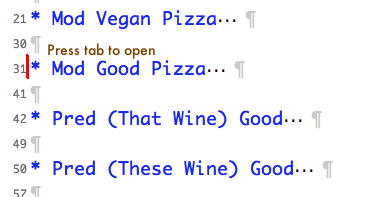
\includegraphics[width=0.6\linewidth]{img/instruction-1.png}

  Place cursor to the left and click tab to open it.
\item
  You get a list of contexts for the test case. Keep the cursor where it
  was if you want to open everything at the same time. Alternatively,
  scroll down to one of the contexts and press tab there, if you only
  want to open one.

  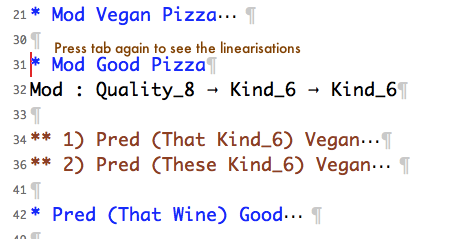
\includegraphics[width=0.7\linewidth]{img/instruction-2.png}
\item

  Now you can read the linearisations.

  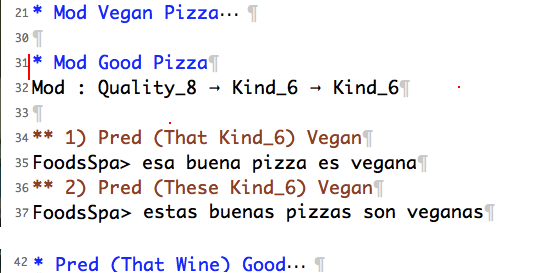
\includegraphics[width=0.75\linewidth]{img/instruction-3.png}
\end{enumerate}

If you want to close the test case, just press tab again, keeping the
cursor where it's been all the time (line 31 in the pictures).

\hypertarget{less-common-use-cases}{%
\subsection{Less common use cases}\label{less-common-use-cases}}

\hypertarget{empty-or-always-identical-fields--e--q}{%
\subsubsection{\texorpdfstring{Empty or always identical fields:
\texttt{-e},
\texttt{-q}}{Empty or always identical fields: -e, -q}}\label{empty-or-always-identical-fields--e--q}}

Information about the fields: always empty, or always equal to each
other. Example of empty fields:

\begin{verbatim}
> gftest -g Lang -l Dut -e
* Empty fields:
==> Ant: s
==> Pol: s
==> Temp: s
==> Tense: s
==> V: particle, prefix
\end{verbatim}

The categories \texttt{Ant}, \texttt{Pol}, \texttt{Temp} and
\texttt{Tense} are as expected empty; there's no string to be added to
the sentences, just a parameter that \emph{chooses} the right forms of
the clause.

\texttt{V} having empty fields \texttt{particle} and \texttt{prefix} is
in this case just an artefact of a small lexicon: we happen to have no
intransitive verbs with a particle or prefix in the core 300-word
vocabulary. But a grammarian would know that it's still relevant to keep
those fields, because in some bigger application such a verb may show
up.

On the other hand, if some other field is always empty, it might be a
hint for the grammarian to remove it altogether.

Example of equal fields:

\begin{verbatim}
> gftest -g Lang -l Dut -q
* Equal fields:
==> RCl:
s Pres Simul Pos Utr Pl
s Pres Simul Pos Neutr Pl

==> RCl:
s Pres Simul Neg Utr Pl
s Pres Simul Neg Neutr Pl

==> RCl:
s Pres Anter Pos Utr Pl
s Pres Anter Pos Neutr Pl

==> RCl:
s Pres Anter Neg Utr Pl
s Pres Anter Neg Neutr Pl

==> RCl:
s Past Simul Pos Utr Pl
s Past Simul Pos Neutr Pl
…
\end{verbatim}

Here we can see that in relative clauses, gender does not seem to play
any role in plural. This could be a hint for the grammarian to make a
leaner parameter type, e.g.
\texttt{param\ RClAgr\ =\ SgAgr\ \textless{}everything\ incl.\ gender\textgreater{}\ \textbar{}\ PlAgr\ \textless{}no\ gender\ here\textgreater{}}.

\hypertarget{unused-fields--u}{%
\subsubsection{\texorpdfstring{Unused fields:
\texttt{-u}}{Unused fields: -u}}\label{unused-fields--u}}

These fields are not empty, but they are never used in the top category.
The top category can be specified by \texttt{-s}, otherwise it is the
default start category of the grammar.

Note that if you give a start category from very low, such as
\texttt{Adv}, you get a whole lot of categories and fields that
naturally have no way of ever making it into an adverb. So this is
mostly meaningful to use for the start category.

\hypertarget{erased-trees--r}{%
\subsubsection{\texorpdfstring{Erased trees:
\texttt{-r}}{Erased trees: -r}}\label{erased-trees--r}}

Show trees that are erased in some function, i.e.~a function
\texttt{F\ :\ A\ -\textgreater{}\ B\ -\textgreater{}\ C} has arguments A
and B, but doesn't use one of them in the resulting tree of type C. This
is usually a bug.

Example:

\begin{verbatim}
> gftest -g Lang -l "Dut Eng" -r

* Erased trees:

** RelCl (ExistNP something_NP) : RCl
- Tree:  AdvS (PrepNP with_Prep (RelNP (UsePron it_Pron) (UseRCl (TTAnt TPres ASimul) PPos (RelCl (ExistNP something_NP))))) (UseCl (TTAnt TPres ASimul) PPos (ExistNP something_NP))
- Lin:   ermee is er iets
- Trans: with it, such that there is something, there is something

** write_V2 : V2
- Tree:  AdvS (PrepNP with_Prep (PPartNP (UsePron it_Pron) write_V2)) (UseCl (TTAnt TPres ASimul) PPos (ExistNP something_NP))
- Lin:   ermee is er iets
- Trans: with it written there is something
\end{verbatim}

In the first result, an argument of type \texttt{RCl} is missing in the
tree constructed by \texttt{RelNP}, and in the second result, the
argument \texttt{write\_V2} is missing in the tree constructed by
\texttt{PPartNP}. In both cases, the English linearisation contains all
the arguments, but in the Dutch one they are missing. (This bug is
already fixed, just showing it here to demonstrate the feature.)

\hypertarget{detailed-information-about-the-grammar}{%
\subsection{Detailed information about the
grammar}\label{detailed-information-about-the-grammar}}

\hypertarget{debug-information--d}{%
\subsubsection{\texorpdfstring{Debug information:
\texttt{-d}}{Debug information: -d}}\label{debug-information--d}}

When combined with \texttt{-f}, \texttt{-c} or \texttt{-t}, two things
happen:

\begin{enumerate}
\def\labelenumi{\arabic{enumi})}
\tightlist
\item
  The trees are linearised using \texttt{tabularLinearize}, which shows
  the inflection table of all forms.
\item
  You can see traces of pruning that happens in testing functions:
  contexts that are common to several concrete categories are put under
  a separate test case.
\end{enumerate}

When combined with \texttt{-\/-show-cats}, also the concrete categories
are shown.

\hypertarget{show-cats}{%
\subsubsection{-\/-show-cats}\label{show-cats}}

Shows the categories in the grammar. With
\texttt{-\/-debug}/\texttt{-d}, shows also concrete categories.

Example:

\begin{verbatim}
> gftest -g Foods -l Spa --show-cats -d

* Categories in the grammar:
Comment
    Compiles to concrete category   0
Item
    Compiles to concrete categories 1—4
Kind
    Compiles to concrete categories 5—6
Quality
    Compiles to concrete categories 7—8
Question
    Compiles to concrete category   9
\end{verbatim}

\hypertarget{show-funs}{%
\subsubsection{-\/-show-funs}\label{show-funs}}

Shows the functions in the grammar. (Nothing fancy happens with other
flags.)

\hypertarget{show-coercions}{%
\subsubsection{-\/-show-coercions}\label{show-coercions}}

First I'll explain what \emph{coercions} are, then why it may be
interesting to show them. Let's take a Spanish Foods grammar, and
consider the category \texttt{Quality}, e.g. \texttt{Good} and
\texttt{Vegan}. \texttt{Good} ``bueno/buena/buenos/buenas'' goes before
the noun it modifies, whereas \texttt{Vegan} ``vegano/vegana/\ldots{}''
goes after, so these will become different \emph{concrete categories} in
the PGF: \texttt{Quality\_before} and \texttt{Quality\_after}. (In
reality, they are something like \texttt{Quality\_7} and
\texttt{Quality\_8} though.)

Now, this difference is meaningful only when the adjective is modifying
the noun: ``la buena pizza'' vs. ``la pizza vegana''. But when the
adjective is in a predicative position, they both behave the same: ``la
pizza es buena'' and ``la pizza es vegana''. For this, the grammar
creates a \emph{coercion}: both \texttt{Quality\_before} and
\texttt{Quality\_after} may be treated as \texttt{Quality\_whatever}. To
save some redundant work, this coercion \texttt{Quality\_whatever}
appears in the type of predicative function, whereas the modification
function has to be split into two different functions, one taking
\texttt{Quality\_before} and other \texttt{Quality\_after}.

Now you know what coercions are, this is how it looks like in the
program:

\begin{verbatim}
> gftest -g Foods -l Spa --show-coercions
* Coercions in the grammar:
Quality_7--->_11
Quality_8--->_11
\end{verbatim}

(Just mentally replace 7 with \texttt{before}, 8 with \texttt{after} and
11 with \texttt{whatever}.)

\hypertarget{show-contexts}{%
\subsubsection{-\/-show-contexts}\label{show-contexts}}

Show contexts for a given concrete category, given as an FId (i.e.~Int).
The concrete category may be a coercion or a normal category. By
combining with
\protect\hyperlink{start-category-for-context--s}{\texttt{-s}}, you can
change the start category of the context.
(You can get a list of all concrete categories by pairing
\texttt{-\/-show-cats} with \texttt{-\/-debug}: see
\protect\hyperlink{--show-cats}{\texttt{-\/-show-cats}}.)

Examples:

\begin{itemize}
\tightlist
\item
  First, find out some concrete categories:
\end{itemize}

\begin{verbatim}
    > gftest -g Foods -l Spa --show-cats -d
    …
    Quality
        Compiles to concrete categories 7—8
    …
\end{verbatim}

\begin{itemize}
\tightlist
\item
  Then, list the contexts for some of them, say \texttt{Quality\_7}:
\end{itemize}

\begin{verbatim}
    > gftest -g Foods -l Spa --show-contexts 7

    Pred (That (Mod ∅ Wine)) Vegan
    Pred (That Wine) ∅
    Pred (These (Mod ∅ Wine)) Vegan
    Pred (These Wine) ∅
    Pred (That (Mod ∅ Pizza)) Vegan
    Pred (That Pizza) ∅
    Pred (These (Mod ∅ Pizza)) Vegan
    Pred (These Pizza) ∅
\end{verbatim}

\begin{itemize}
\item
  You can also give it a range of arguments, with starting and ending
  category in quotes:
  \texttt{gftest\ -g\ Foods\ -l\ Spa\ -\/-show-contexts\ "7\ 10"}
\item
  Check out from
  \protect\hyperlink{--show-coercions}{\texttt{-\/-show-coercions}} how
  to find coercions, and you can try \texttt{-\/-show-contexts} with
  them:
\end{itemize}

\begin{verbatim}
    > gftest -g Foods -l Spa --show-contexts 11

    Pred (That Wine) ∅
    Pred (These Wine) ∅
    Pred (That Pizza) ∅
    Pred (These Pizza) ∅
\end{verbatim}

\hypertarget{count-trees}{%
\subsubsection{-\/-count-trees}\label{count-trees}}

Number of trees up to given size. Gives a number how many trees, and a
couple of examples from the highest size. Examples:

\begin{verbatim}
> gftest -g TestLang -l Eng --count-trees 10
There are 675312 trees up to size 10, and 624512 of exactly size 10.
For example:
* AdvS today_Adv (UseCl (TTAnt TPres ASimul) PPos (ExistNP (UsePron i_Pron)))
* UseCl (TTAnt TCond AAnter) PNeg (PredVP (SelfNP (UsePron they_Pron)) UseCopula)
\end{verbatim}

This counts the number of trees in the start category. You can also
specify a category:

\begin{verbatim}
> gftest -g TestLang -l Eng --count-trees 4 -s Adv
There are 2409 trees up to size 4, and 2163 of exactly size 4.
For example:
* AdAdv very_AdA (PositAdvAdj young_A)
* PrepNP above_Prep (UsePron they_Pron)
\end{verbatim}

\hypertarget{funs-of-arity}{%
\subsubsection{-\/-funs-of-arity}\label{funs-of-arity}}

Show all functions of given arity (not up to).

Example:

\begin{verbatim}
> gftest -g Phrasebook --funs-of-arity 3
* Functions in the grammar of arity 3:
ADoVerbPhrasePlace
AModVerbPhrase
HowFarFromBy
QWhereModVerbPhrase
\end{verbatim}
